%!TEX root=masterproef.tex

\chapter{Inleiding}
\label{inleiding}

Ofschoon de naam nog geen gemeengoed is, is de opmars van draadloze
sensornetwerken (DSN) in ons dagelijks leven niet meer te stoppen. Na de
revolutie van de persoonlijke computer, de smartphone en het tablet vinden nu
onafhankelijke, minuscule computers hun weg naar allerlei alledaagse dingen en
plaatsen in ons leven. Met hun sensoren kunnen ze de kleinste wijzigingen in
hun omgeving optekenen en via een draadloos netwerk staan ze in verbinding met
elkaar en de buitenwereld. Zo leveren ze hun informatie af, waardoor wij op elk
moment precies weten hoe warm het in elke kamer in ons huis is of welke
groenten we nog in de koelkast hebben liggen. Het lijkt soms nog science
fictie, maar de toekomst is al heel wat dichterbij dan we soms denken.

Indien we deze technologie willen omarmen en ons leven verder willen inrichten
met al deze fantastische ondersteunende hulp, moeten we ons er wel van
vergewissen dat deze technologie betrouwbaar en veilig is. Als enkele sensoren
in ons huis slechts een kleine stap met weinig potenti\"ele, problematische
gevolgen lijkt, moeten we ons misschien toch maar eens bezinnen en beseffen dat
al deze kleine computers met hun sensoren wel eens zeer interessante
mogelijkheden bieden aan anderen met minder positieve bedoelingen.

Misschien wil de concurrent van de producent van onze yoghurt zijn collega wel
in diskrediet brengen door er voor te zorgen dat onze slimme koelkast het
nalaat ons te verwittigen dat het potje yoghurt al een week vervallen is.
Misschien vindt de gasleverancier het wel leuk om overdag, wanneer we niet
thuis zijn, de thermostaat een graadje hoger te zetten. 

De mogelijkheden die draadloze sensornetwerken met zich meebrengen zijn zonder
twijfel fantastisch en ze kunnen de kwaliteit van ons leven ingrijpen
veranderen. Ze mogen echter geen nieuwe bedreiging introduceren. In deze
masterproef duiken we in de wereld van draadloze sensornetwerken en willen we
nagaan of en hoe we deze kunnen voorzien van voldoende bescherming tegen zij
met minder goede bedoelingen.

In dit eerste hoofdstuk introduceren we draadloze sensornetwerken. Hoe zijn ze
opgebouwd? Wat zijn hun mogelijkheden en beperkingen? (\ref{section:wsn}) Wat
zijn de gevaren waaraan ze blootgesteld zijn? Hoe kunnen deze gevaren
vastgesteld worden? Hoe kunnen sensorknopen tegen deze gevaren beschermd
worden? (\ref{section:beveiligen})

Verder defini\"eren we het probleem dat we willen aanpakken
(\ref{section:probleem}) en stellen onze doelstelling voor
(\ref{section:doelstelling}). Na dit hoofdstuk liggen alle speelstukken op
tafel.

\section{Draadloze sensornetwerken}
\label{section:wsn}

Sinds de late jaren '90 zijn draadloze sensornetwerken een bron geweest voor
een explosie aan onderzoek. Binnen en buiten universiteiten werden deze
netwerken ingezet voor allerhande toepassingen: van het opvolgen van
microklimaten bij het telen van gewassen door \cite{baggio2005wireless} tot het
vastleggen van vulkanische activiteit \cite{werner2005monitoring} of het
opvolgen van overstromingsgebieden \cite{hughes2006gridstix}.

Wat moeten we ons eigenlijk voorstellen bij een draadloos sensornetwerk? We
bekijken kort de sensorknopen, waarmee het netwerk wordt opgebouwd. Vervolgens
belichten we het draadloze netwerk dat de knopen in staat stelt om met elkaar
en met de buitenwereld te communiceren.

\subsection{Sensorknopen}

Sensorknopen zijn in essentie zeer eenvoudige computers. Ze worden typisch
opgebouwd rond een microcontroller (\mcu). Dit is een digitaal ontwerp dat
zowel een processor, als geheugen en invoer- en uitvoerkanalen bevat op \'e\'en
enkele ge\"integreerde schakeling. Ze worden daarom ook wel
\emph{systeem-op-een-chip} genoemd. Figuur \ref{fig:motes} toont enkele
typische sensorknopen.

\begin{figure}[h]
\centering
\begin{subfigure}{.24\textwidth}
  \centering
  \includegraphics[width=.9\linewidth]{./resources/mica2.jpg}
  \caption{Mica2}
  \label{fig:mica2}
\end{subfigure}
\begin{subfigure}{.24\textwidth}
  \centering
  \includegraphics[width=.9\linewidth]{./resources/dot.png}
  \caption{Dot}
  \label{fig:dot}
\end{subfigure}
\begin{subfigure}{.24\textwidth}
  \centering
  \includegraphics[width=.9\linewidth]{./resources/telos.jpg}
  \caption{Telos}
  \label{fig:telos}
\end{subfigure}
\begin{subfigure}{.24\textwidth}
  \centering
  \includegraphics[width=.9\linewidth]{./resources/raven.jpg}
  \caption{AVRraven}
  \label{fig:raven}
\end{subfigure}
\caption{Voorbeelden van sensorknopen.}
\label{fig:motes}
\end{figure}

Naast de \mcu heeft een typische sensorknoop tevens een draadloze radio. Je kan
dit vergelijken met de Wi-Fi verbinding die je tegenwoordig in de meeste
computers of smartphones vindt. Voor sensorknopen wordt echter meestal
geopteerd voor een draadloze radio die een minimum aan energie probeert te
verbruiken. Verschillende nieuwe draadloze netwerkstandaarden zijn de laatste
jaren op het voortouw getreden. De bekendste zijn 6LoWPAN \cite{rfc:6282} en
ZigBee \cite{alliance2012zigbee}. Voor deze masterproef kozen we ZigBee als
technische draadloze standaard. In de volgende paragrafen bekijken we de manier
waarop deze standaard opgebouwd is en werkt, enerzijds omwille van de
toepassing in deze masterproef, maar anderzijds ook wegens de voorbeeldfunctie
die de standaard kan aannemen voor deze groep van draadloze standaarden.

\subsection{ZigBee}
\label{subsection:zigbee}

ZigBee zelf is slechts een laag bovenop de netwerklaag gekend als IEEE 802.15.4
\cite{ieee2009802.15.4}. Deze laag voorziet standaarden op vlak van
energiegebruik, adressering, foutcorrectie, vormgeving van berichten,\dots en
vormt zo de fundamenten voor \emph{low-rate wireless personal area networks}
(LR-WPAN). Bovenop deze laag voegt ZigBee nog drie belangrijke eigenschappen:
routering, ad-hoc netwerk creatie en zelfherstellende maasnetwerken
\cite{oreilly2010buildingwsn}.

Een ZigBee netwerk wordt opgebouwd door knopen die elk \'e\'en van drie
verschillende functies kunnen innemen: co\"ordinator, router of eindknoop. Elk
netwerk heeft precies \'e\'en \emph{co\"ordinator}. Deze knoop is
verantwoordelijk voor het samenbrengen van het netwerk en definieert de
parameters van het netwerk, bv. met betrekking tot de beveiliging.

Een \emph{router} stelt andere knopen in staat om met elkaar te communiceren.
Deze knopen zijn daarom meestal voorzien van een permanente stroomvoorziening,
omdat ze in tegenstelling tot \emph{eindknopen}, zich niet in een slaapstand
kunnen zetten, wegens hun communicatieondersteunende rol.

\emph{Eindknopen}, tot slot, kunnen zich louter verbinden met een netwerk en er
berichten naartoe sturen. Ze kunnen geen berichten van andere knopen voor
andere knopen ontvangen en doorsturen. Typisch trachten ze ook hun
energieverbruik te minimaliseren door hun draadloze radio zoveel mogelijk uit
te schakelen. Hierdoor worden ze onbereikbaar. Het is dankzij de \emph{routers}
die berichten voor de \emph{eindknopen} tijdelijk opslaan, dat deze
\emph{eindknopen} toch alle berichten kunnen ontvangen.

\subsection{Netwerk topologie en adressen}
\label{subsection:topologie}

Met knopen kunnen verschillende netwerk topologie\"en gebouwd worden. Figuur
\ref{fig:topologie} geeft een overzicht van de mogelijkheden. In zijn
eenvoudigste vorm bestaat een netwerk uit een co\"ordinator en een eindknoop.
Wanneer meerdere eindknopen verbonden zijn met dezelfde co\"ordinator, vormen
zij een stertopologie. Alle communicatie verloopt via de centrale
co\"ordinator. In een maasnetwerk, worden routers ingeschakeld om communicatie
via verschillende wegen mogelijk te maken. Eindknopen zijn verbonden met deze
routers of de co\"ordinator, routers en de co\"ordinator kunnen berichten
ontvangen van eindknopen en deze versturen naar andere eindknopen, al dan niet
via andere routers. Een speciale vorm van een maasnetwerk is een clusterboom.
Hierbij vormen groepen van eindknopen en een router een cluster. De router is
verbonden met de co\"ordinator, eventueel opnieuw via andere routers, en zo
wordt een boomstructuur gevormd. De routers die de clusters van eindknopen
realiseren worden ook clusterhoofden genoemd.

\begin{figure}
  \centering
  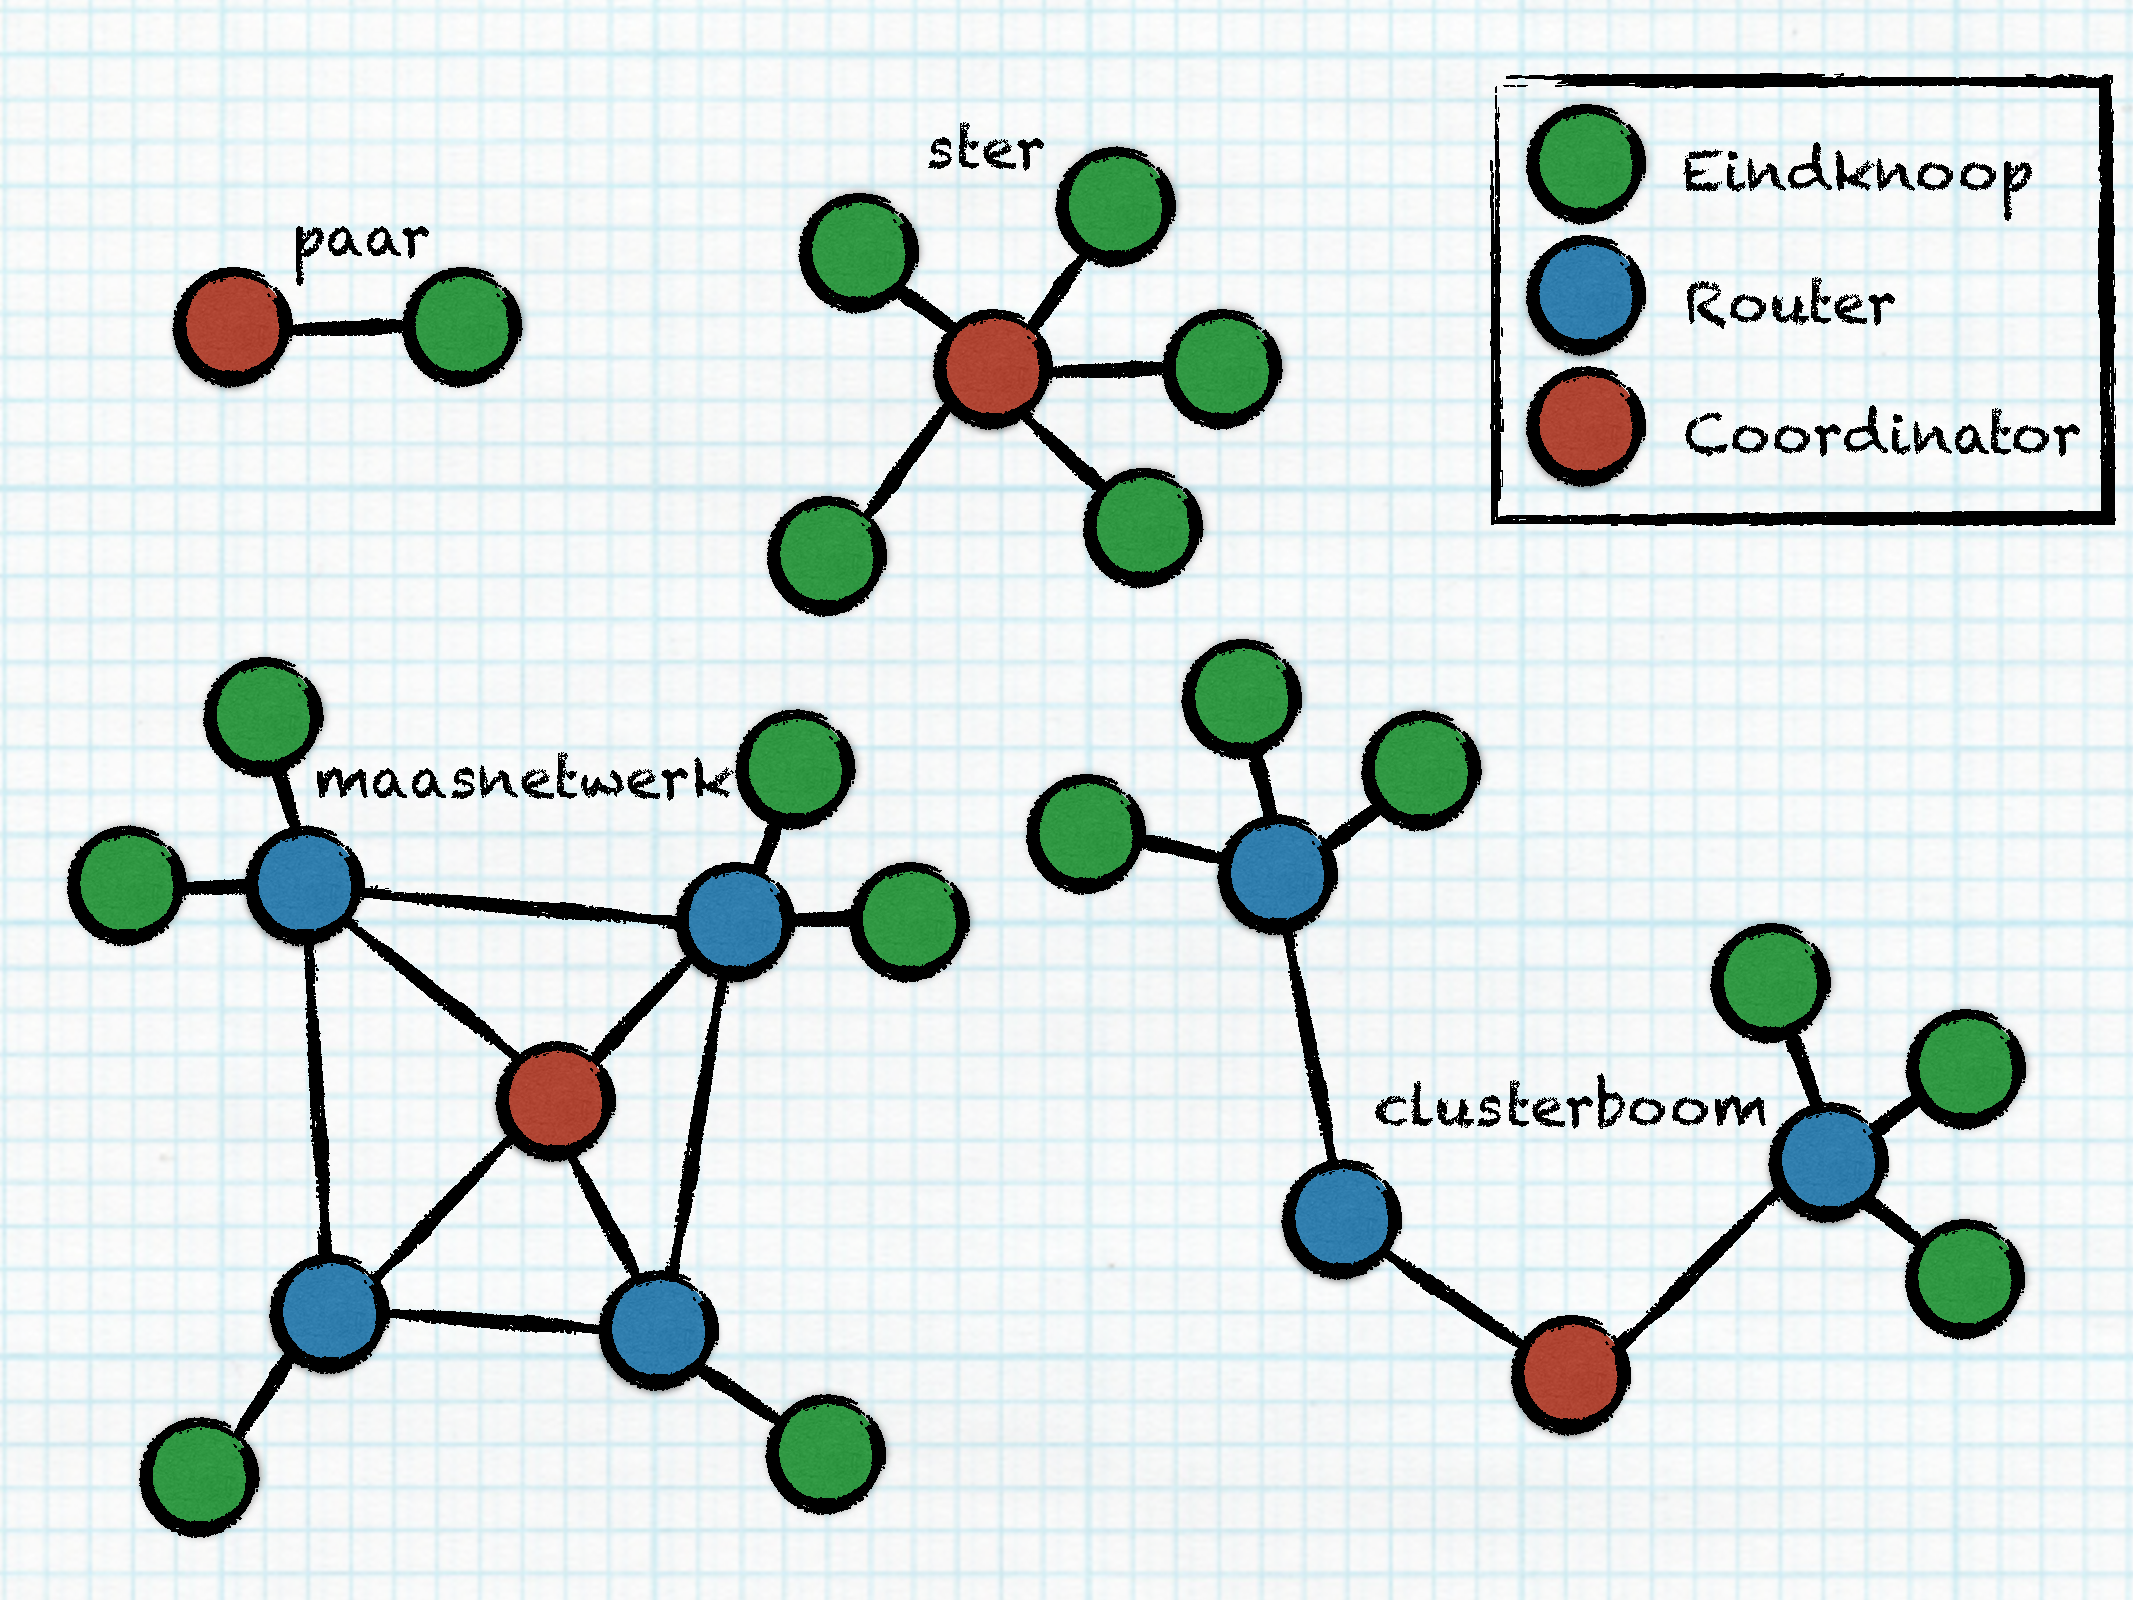
\includegraphics[width=0.7\linewidth]{resources/topology.pdf}
  \caption{Verschillende mogelijke netwerktoplogie\"en.}
  \label{fig:topologie}
\end{figure}

Het lijkt evident, maar elke knoop, in eender welke topologie, heeft een eigen,
uniek adres. Eigenlijk meerdere. Zo heeft een ZigBee knoop een uniek adres
binnen het netwerk waaraan het deelneemt. Dit adres wordt door de co\"ordinator
van het netwerk toegekend aan een knoop wanneer deze toetreedt tot het netwerk.
Dit \emph{netwerk adres} bestaat uit 16 bits en laat dus toe om 65534
verschillende adressen toe te kennen. Het adres 0000\footnote{We hanteren voor
de notatie van adressen de hexadecimale voorstelling. Elk cijfer stelt een
groep van 4 bits voor. 4 groepen stellen zo een 16 bit adres voor.} reserveert
de co\"ordinator voor zichzelf en het adres FFFE wordt typisch gebruikt als het
zgn. \emph{broadcast adres}, het adres waarnaar een bericht gestuurd wordt dat
bij alle andere knopen dient afgeleverd te worden.

Maar daarnaast heeft elke ZigBee radio ook een eigen, unieke adres dat
gegarandeerd overal uniek is. Dit adres bestaat uit 64 bits en wordt
samengesteld uit een hoog en laag gedeelte. Het hoge gedeelte beslaat de eerste
32 bits en is voorbehouden voor de unieke identificatie van de producent van de
radio. De lage reeks van 32 bits is een uniek nummer binnen de productie van de
producent. Het is daarom logisch dat er gebruik gemaakt wordt van een
\emph{netwerk adres}, dat slechts 16 bits groot is en dus een aanzienlijke
besparing aan geheugen kan opleveren.

Naast de adressen van de knopen is er ook nog het zogenaamde \emph{personal
area network (PAN)} adres. Dit is een unieke identificatie van het netwerk dat
door de co\"ordinator georganiseerd wordt. Ook dit is een 16 bit adres en laat
dus toe om 65536 netwerken op te bouwen.

Tot slot kunnen ZigBee radio's ook gebruik maken van 12 verschillende kanalen,
zodat de volledige adresstructuur bestaat uit een kanaal, een PAN adres en een
netwerk adres.

\section{Beveiligen van sensorknopen}
\label{section:beveiligen}

Het beveiligen van sensorknopen is in tegenstelling tot de beveiliging van
klassieke computers een bijzonder moeilijke aangelegenheid. De computers waar
onze emails, foto's en andere kostbare documenten opgeslagen zijn, zijn
uitgerust met een virusscanner, firewall,\dots. Dit is mogelijk omdat ze
voorzien zijn van een constante stroomvoorziening. Ze zijn tevens beschermd
door ons huis of het datacenter van onze leverancier van internetdiensten.

In \cite{dargie2010fundamentals} wordt een goed overzicht gegeven van de
uitdagingen die het beveiligen van DSN met zich meebrengen, in tegenstelling
tot de klassieke situatie. Een sensorknoop heeft geen constante
stroomvoorziening en moet het veelal stellen met een zeer beperkte batterij.
Verder ligt de sensorknoop meestal letterlijk \emph{ten velde} en is fysiek
toegankelijk voor nagenoeg iedereen.

Verder is er geen centraal punt waar alle communicatie van en naar de
sensorknoop gegarandeerd passeert. Het enige communicatiemedium is het
draadloze netwerk en via die weg kan men steeds rechtstreeks contact leggen met
elke afzonderlijke knoop, zonder dat een andere knoop dit ooit merkt. Tot slot
is het belangrijk dit nog aan te vullen met het feit dat een draadloos
communicatiemedium inherent fouten met zich meebrengt, en dat berichte verloren
kunnen gaan.

\subsection{CIA en andere beveiligingsprincipes}
\label{subsection:cia}

Wanneer men spreekt over het beveiligen van computers en netwerken, wordt
veelal gerefereerd naar het CIA beveiligingsmodel. Dit letterwoord staat voor:
vertrouwelijkheid (Engels: \emph{confidentiality}), integriteit en
beschikbaarheid (Engels: \emph{availability}).

Om \emph{Vertrouwelijkheid} te garanderen moet beveiliging de nodige
voorzieningen treffen om er voor te zorgen dat een bericht enkel door de
bedoelde bestemmeling kan begrepen worden. Onder \emph{integriteit} verstaat
men het principe dat een bericht niet kan gewijzigd worden, of dat de bedoelde
bestemmeling van het bericht ten minste als enige kan valideren dat er aan het
bericht niets gewijzigd is. Maar beveiliging moet ook de \emph{beschikbaarheid}
van onderdelen van het netwerk garanderen, om er zeker van te zijn dit laatste
zijn diensten kan blijven aanbieden.

Naast deze drie hoofdpijlers zijn volgende bijkomende principes van belang:
authenticatie, autorisatie en onweerlegbaarheid (Engels: \emph{nonrepudiation}).

Via \emph{authenticatie} kan de identiteit van een gebruiker of apparaat
vastgesteld worden, zodat eenduidig kan bepaald worden van wie bv. een bericht
in het netwerk komt. \emph{Autorisatie} is dan het proces waarbij nagegaan
wordt of een geauthenticeerde gebruiker een bepaalde handeling mag uitvoeren.
Door garanties omtrent \emph{onweerlegbaarheid} in te bouwen, kan bv. een
ontvanger er zeker van zijn dat een zender van een bericht effectief dit
bericht verstuurd heeft. Digitale handtekeningen kunnen typisch helpen bij het
garanderen van authenticatie, onweerlegbaarheid en de integriteit.

\TODO

\subsection{Inbraakdetectie}
\label{subsection:detection}

\TODO

\section{Probleemstelling}
\label{section:probleem}

\TODO

\section{Doelstelling}
\label{section:doelstelling}

In de literatuur betreffende ``inbraakdetectie in draadloze sensornetwerken'',
ligt de nadruk in hoofdzaak op het detecteren van specifieke aanvallen of het
vaststellen van anomalie\"en in het verwachte gedrag van sensorknopen en/of het
netwerk dat hen verbindt.

Deze werken stellen tevens dat het een nagenoeg onmogelijke taak is om alle
benodigde detectiemechanismen effectief te implementeren. Dit is logisch
gegeven het beperkte aanbod aan middelen die sensorknopen typisch ter hunnen
beschikking hebben. Zo zou bv. een exhaustieve lijst van aanvalspatronen
slechts in sensorknopen met zeer grote hoeveelheden geheugen kunnen opgeslagen
worden en zouden de berekeningen die nodig zijn om verschillende anomalie\"en
te detecteren gewoonweg te veel energie verbruiken.

Als in deze fase van onderzoek naar systemen om inbraken te detecteren het niet
mogelijk is om een sluitend intrusie detectie systeem voor draadloze
sensornetwerken te ambi\"eren, lijkt het opportuun om een stap terug te nemen
en de focus eerst te leggen op de middelen die nodig zijn om de reeds
beschreven en mogelijk ook toekomstige oplossingen te realiseren. Is het
mogelijk om een raamwerk te cre\"eren dat een ontwikkelaar van een sensorknoop
in staat stelt om een selectie van de in de literatuur beschreven oplossingen
te implementeren, zonder zich zorgen te moeten maken over de onderliggende
interactie met andere knopen, het vergaren en opvragen van informatie op
systeem-niveau,...?

Deze thesis wil zulk een raamwerk ontwerpen, implementeren en de impact ervan
bepalen. Daartoe zal eerst een lijst gemaakt worden van de verwerkte
oplossingen, waaruit de functionele en technische vereisten voor het raamwerk
gedistilleerd kunnen worden. Vervolgens zal een architectuur voorgesteld worden
die aan deze vereisten voldoet. Aan de hand van een implementatie van deze
architectuur zal tot slot nagegaan worden wat de impact is van dit raamwerk met
betrekking tot geheugen en rekenkracht.

De voordelen van zulk een raamwerk zijn legio: een herbruikbaar raamwerk neemt
zorgen, gemeenschappelijk aan de verschillende oplossingen weg en kan zorgen
voor een optimale implementatie. Door middel van een goedgekozen technische
architectuur kan tevens platform-onafhankelijheid nagestreefd worden.
